\section{Discusión}
Este trabajo encuentra que en promedio los agentes tienen expresiones de género acordes a lo socialmente prescrito para su identidad. También encuentra que, en promedio, hay una baja disposición a trabajar en grupo con personas que tenían una vestimenta femenina y reportaban que su habilidad principal eran las matemáticas. Esa baja disposición a trabajar con personas con esas características, puede estar fundamentado en la creencia de que su aporte al desarrollo del meme pudiera ser menor al aporte de personas con otras características. Sin embargo, las personas con vestimenta femenina, hábiles en matemáticas, fueron las que obtuvieron el mejor desempeño (ver figura \ref{fig:performance}). 

\begin{figure}[htbp]
    \centering
    \begin{subfigure}{0.49\textwidth}
        \centering
        \caption{Ranking promedio}
        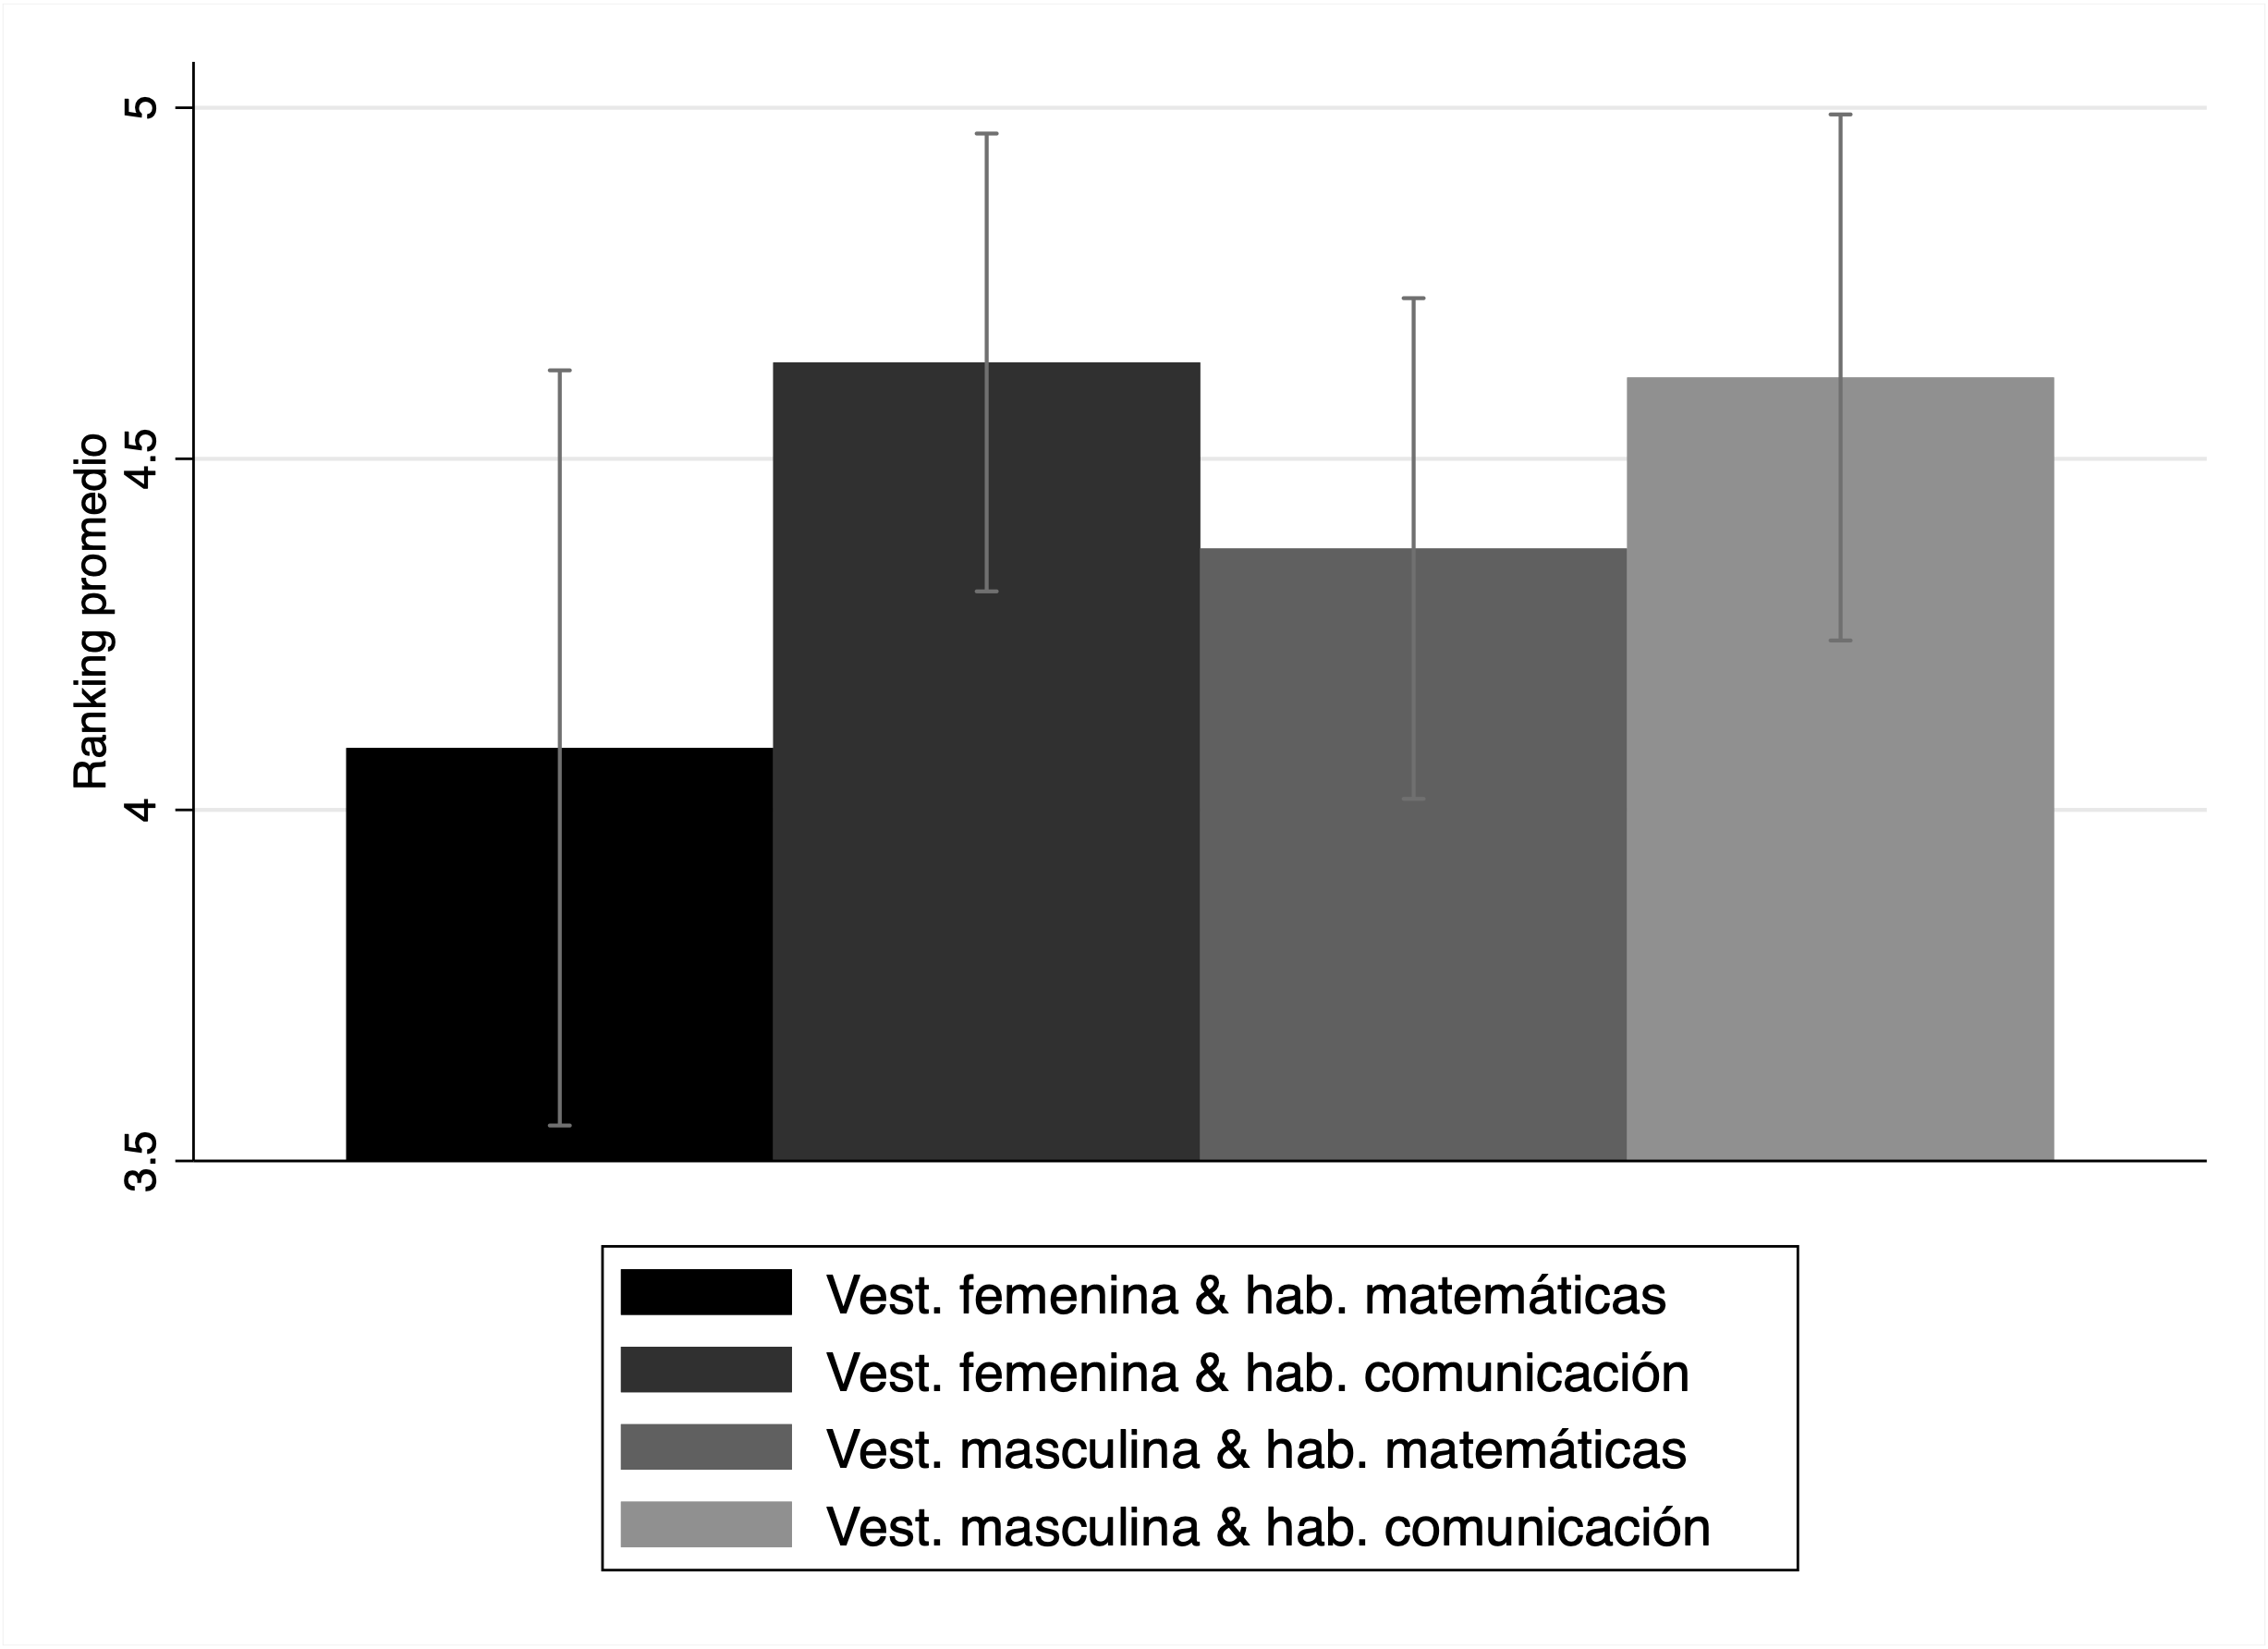
\includegraphics[width=\textwidth]{Images/ranking.png}
    \end{subfigure}
    \begin{subfigure}{0.49\textwidth}
        \centering
        \caption{Desempeño promedio}
        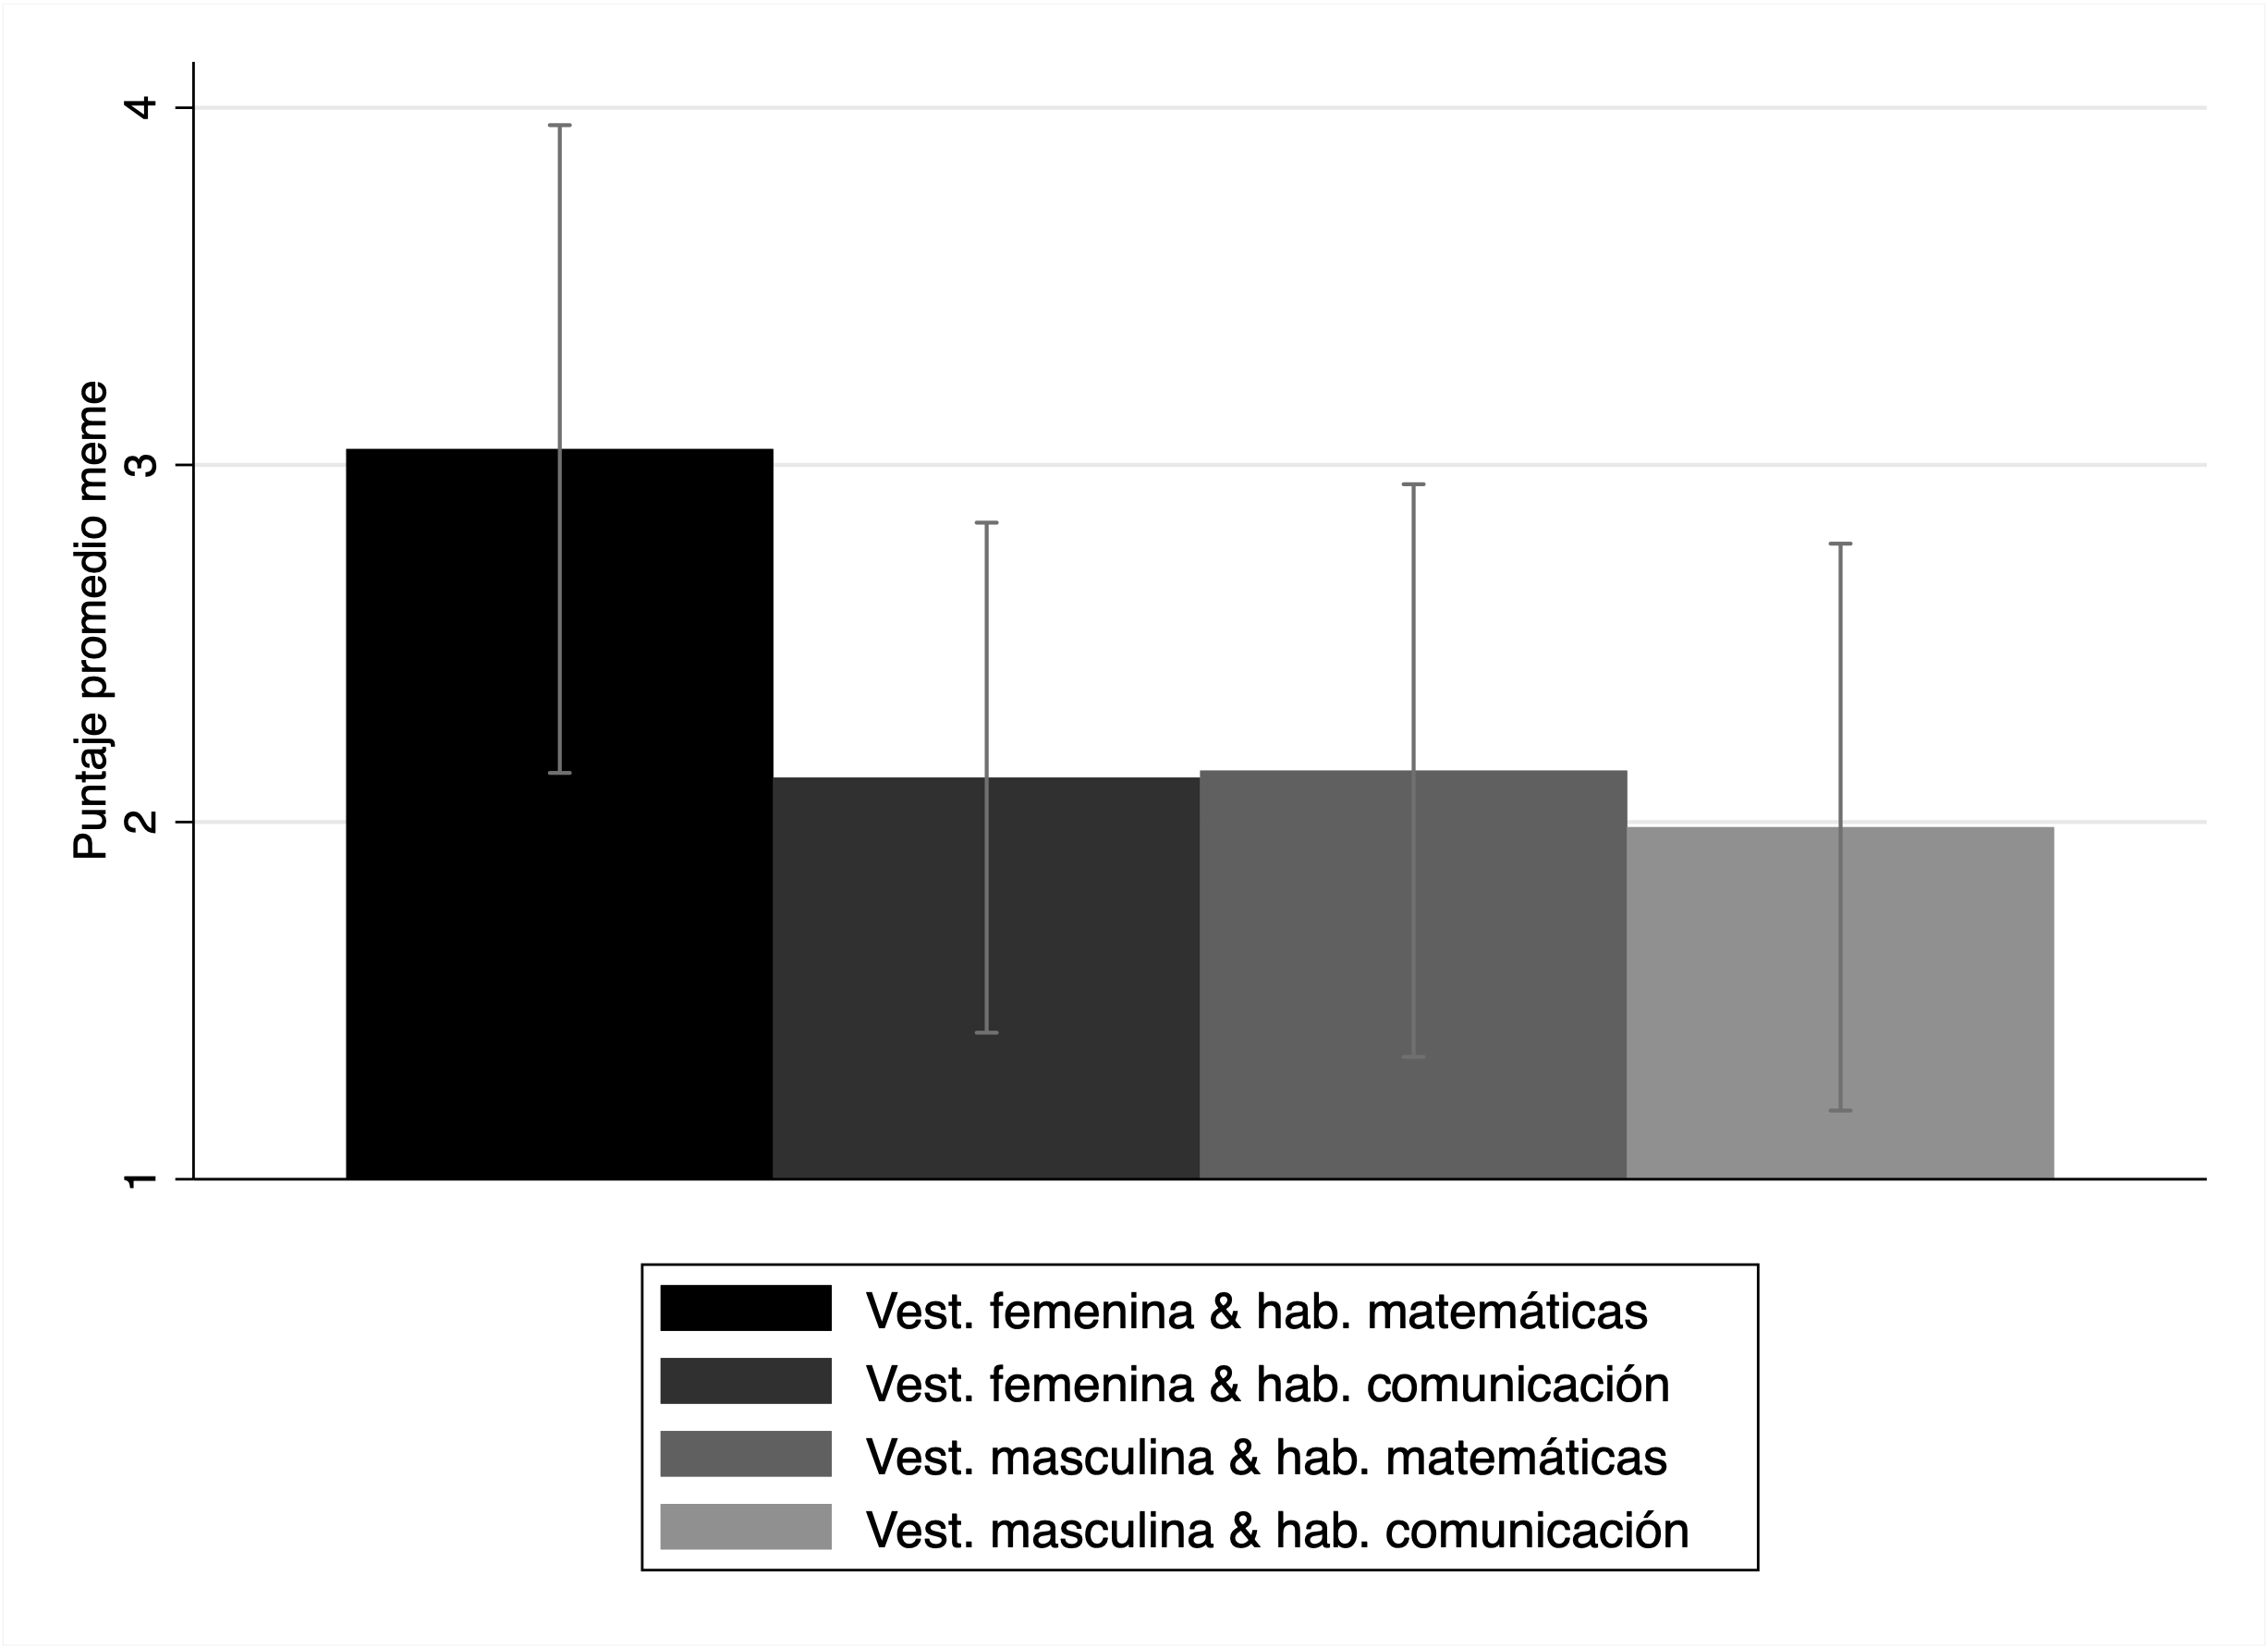
\includegraphics[width=\textwidth]{Images/performance.png}
    \end{subfigure}
    \caption{Ranking y desempeño promedio por conjunto de expresiones de género}
    \label{fig:performance}
    \begin{singlespace}
    \floatfoot{\footnotesize{\textit{Nota:} Gráficas del \textit{ranking} y desempeño promedio. El desempeño promedio corresponde al promedio del puntaje que cada juez le dio al \textit{meme} Intervalos de confianza al 95\%. }\par}
    \end{singlespace}
\end{figure}

El desempeño, definido como el promedio del puntaje (de 0 a 5) que cada juez le dio al \textit{meme}, ignora el aporte de cada persona del grupo al \textit{meme}. Pero, si en efecto existe algún grado de relación entre las características y el desempeño, si la población de participantes se hubiera segmentado entre personas con vestimenta femenina, hábiles en matemáticas y el resto de la población, estos últimos habrían tenido un desempeño subóptimo (inferior al desempeño posible). 
